\documentclass{article}
\usepackage[utf8]{inputenc}
\usepackage[T1]{fontenc}
\usepackage[slovak]{babel}
\usepackage{geometry}
\geometry{a4paper, margin=1in}
\usepackage{hyperref}
\usepackage{graphicx}

\title{Používateľská príručka: Aplikácia Šípka}
\author{Mgr. Lukáš Gajdošech}
\date{}

\begin{document}

\maketitle

\section*{Úvod}
Aplikácia Šípka je interaktívna webová aplikácia určená na riešenie a tvorbu labyrintov pomocou umiestňovania šípok. Umožňuje študentom riešiť labyrinty v režime študenta a učiteľom vytvárať a upravovať labyrinty v režime učiteľa. Aplikácia podporuje načítanie a ukladanie máp, automatické generovanie labyrintov a vizualizáciu riešení.

\section*{Režim študenta (main.html)}

\begin{center}
    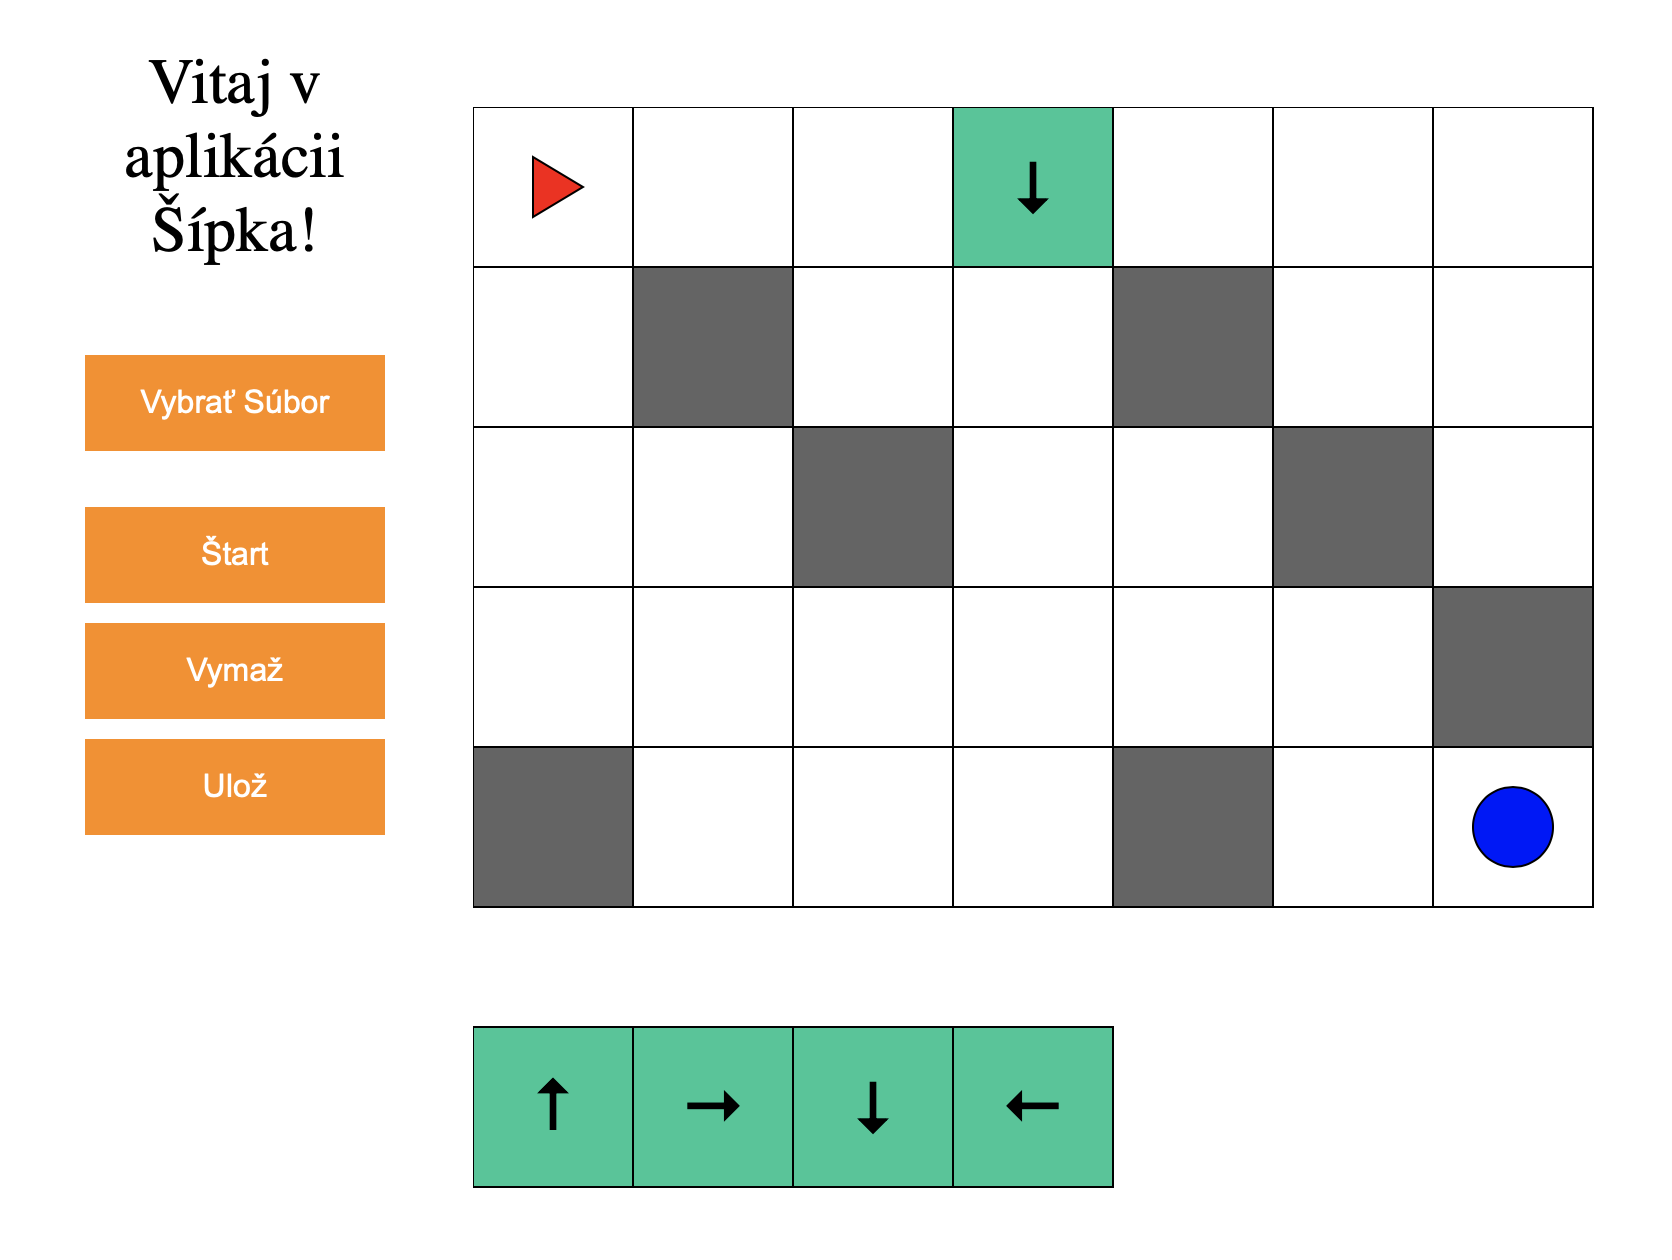
\includegraphics[width=12cm]{student.png}
\end{center}

V režime študenta môžu používatelia interaktívne umiestňovať šípky na hraciu plochu a tým usmerňovať pohyb robota cez labyrint.

\subsection*{Tlačidlá a ich funkcie}
\begin{itemize}
    \item \textbf{Učiteľský Režim}: Prepína aplikáciu do režimu učiteľa.
    \item \textbf{Vybrať Súbor}: Umožňuje načítať labyrint z lokálneho súboru. Tlačidlo spustí dialógové okno pre výber súboru.
    \item \textbf{Štart/Pauza/Pokračuj}: Slúži na spustenie, pozastavenie alebo pokračovanie v riešení labyrintu.
    \item \textbf{Vymaž}: Resetuje aktuálny stav labyrintu a vymaže všetky umiestnené šípky.
    \item \textbf{Ulož}: Umožňuje uložiť aktuálny stav labyrintu do súboru.
    \item \textbf{Riešenie}: Zobrazuje optimálne riešenie labyrintu, ak existuje.
\end{itemize}

\subsection*{Interakcia s aplikáciou}
\begin{itemize}
    \item \textbf{Umiestnenie šípok}: Šípky sa môžu ťahať myšou na hraciu plochu, kde určujú smer pohybu robota.
    \item \textbf{Načítanie a ukladanie máp}: Labyrinty môžu byť načítané zo súborov alebo uložené pre ďalšie použitie.
\end{itemize}

\section*{Režim učiteľa (teacher.html)}

\begin{center}
    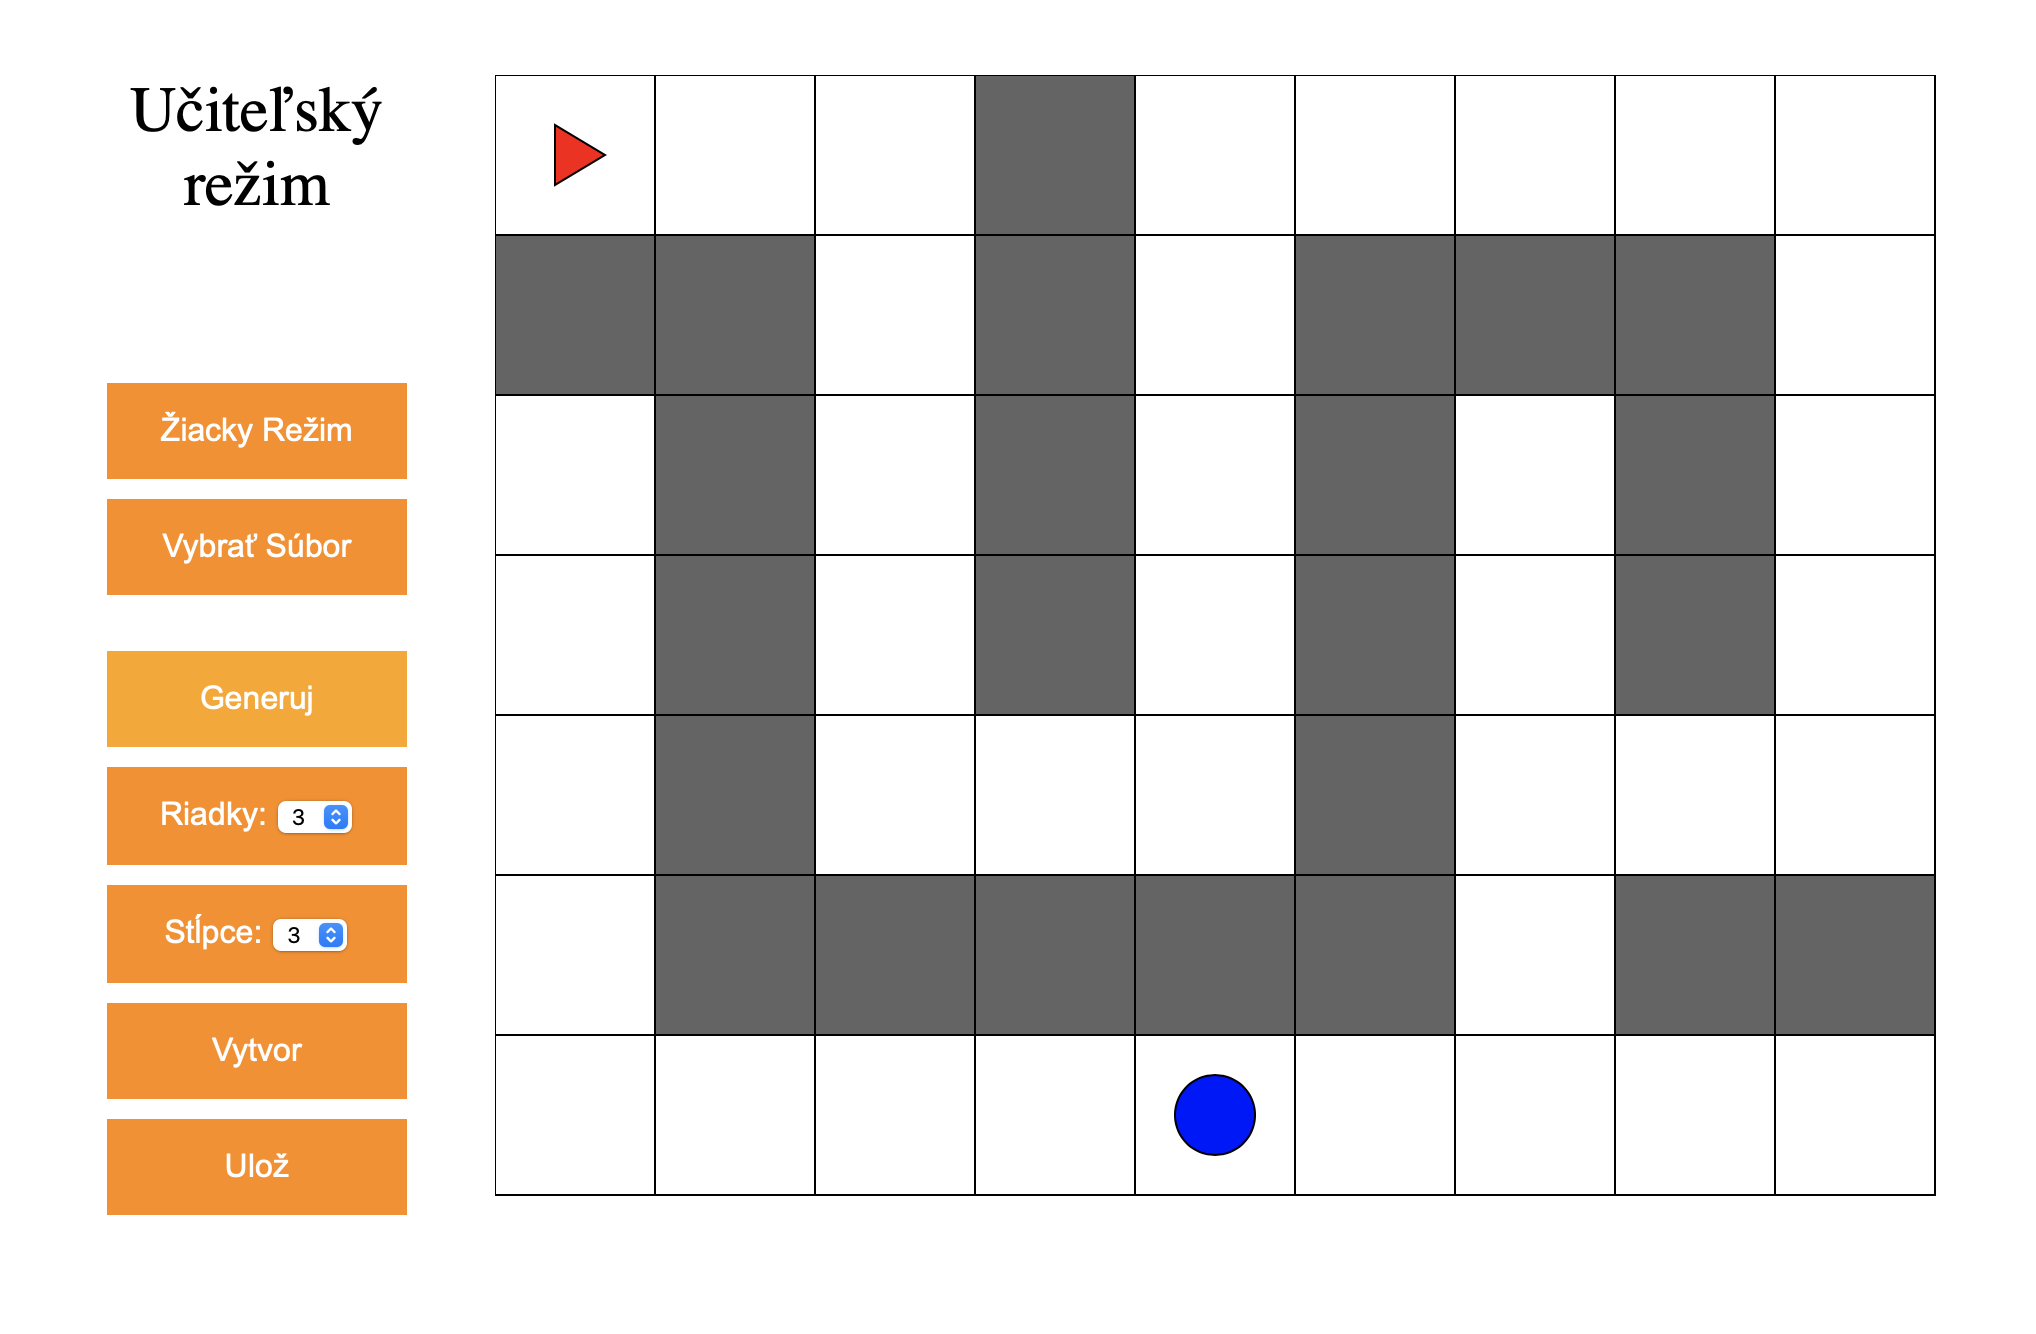
\includegraphics[width=12cm]{teacher.png}
\end{center}

Režim učiteľa poskytuje rozšírené možnosti na tvorbu a úpravu labyrintov, vrátane manuálnej tvorby a automatického generovania.

\subsection*{Tlačidlá a ich funkcie}
\begin{itemize}
    \item \textbf{Generuj}: Automaticky generuje nový labyrint podľa zadefinovaných pravidiel.
    \item \textbf{Manuálne Tvorba}: Umožňuje učiteľovi manuálne pridávať alebo odoberať steny v labyrinte.
    \item \textbf{Ulož}: Umožňuje uložiť vytvorený alebo upravený labyrint do súboru.
\end{itemize}

\subsection*{Interakcia s aplikáciou}
\begin{itemize}
    \item \textbf{Editácia mapy}: Učiteľ môže pridávať alebo odoberať steny v labyrinte kliknutím na príslušné bunky na hracej ploche.
\end{itemize}

\section*{Scenáre použitia}
\begin{itemize}
    \item \textbf{Vzdelávacie účely}: Učitelia môžu vytvárať labyrinty na testovanie logického myslenia študentov.
    \item \textbf{Súťaže}: Študenti môžu súťažiť v rýchlosti riešenia labyrintov.
    \item \textbf{Sebahodnotenie}: Študenti môžu používať aplikáciu na testovanie a zlepšovanie ich schopností riešiť problémy.
\end{itemize}

Táto príručka poskytuje základné informácie o používaní aplikácie Šípka. Pre ďalšie detaily alebo pomoc, kontaktujte vývojárov alebo technickú podporu.

Pre úplnú technickú špecifikáciu aplikácie si prosím prečítajte nasledujúci dokument: \href{https://docs.google.com/document/d/1iO6MmWv0fqi1tS6VNDiRenPgHrlYh8M751RDV6SoXGI/edit?usp=sharing}{Dokument Technickej Špecifikácie}.

\end{document}
